\subsection{Problem definition}

Based on the last benchmark example, the heat transport by advection and diffusion in a fracture, this problem is extended by heat diffusion through a rock matrix orthogonal to the fracture (Fig.~\ref{fig-lauwerier-problem}). 
\begin{figure}[h]
\centering
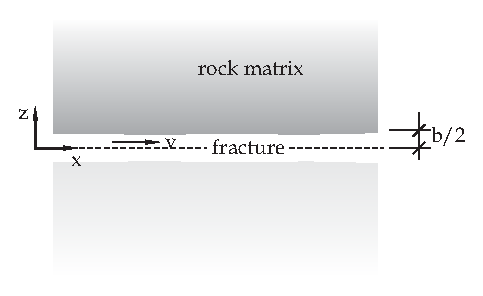
\includegraphics[width=0.5\textwidth]{T/figures/lauwerier-problem.eps}
\caption{\label{fig-lauwerier-problem}Heat transport in a fracture-matrix system.}
\end{figure}
%%%%%%%%%%%%%%%%%%%%%%%%%%%%%%%%%%%%%%%%%%%%%%%%%%%%%%%%%%%%%%%%%%%%%%%%%%%%%%%%%%%%%%%%%%%%%%%%%%%%%%%%%%%%%%%%%%%%
\subsection{Analytical solution}

For this problem an analytical solution is given by \textsc{Lauwerier} (1955) (see \cite{Kol:97}) with following restrictions:
\begin{compactitem}
\item in the fracture, heat is transported just by advection,
\item in the rock matrix, heat transport takes place by diffusion (only along the z-axis).
\end{compactitem}
The \textsc{Lauwerier} equation is given by
\begin{equation}
T_D=\begin{cases}
0, & t_D < x_D \\
\operatorname{erfc}\left\{ \frac{\beta}{\sqrt{\alpha\left(t_D-x_d\right)}} \left[ x_D+\frac{1}{2\beta}\left( z_D-\frac{1}{2} \right) \right]\right\}, & t_D > x_D
\end{cases},   z_D \geq\frac{1}{2}
\label{lauwerier}
\end{equation}
with the following dimensionless parameters:
\begin{equation}
t_D=\frac{v_x}{b}t,\ \ \ x_D=\frac{x}{b},\ \ \ z_D=\frac{z}{b},\ \ \ \alpha =\frac{\lambda ^{r}}{c^{r}\rho ^{r}}\frac{1}{bv_x},\ \ \ \beta = \frac{\lambda^{r}}{c^{w}\rho^{w}}\frac{1}{bv_x}
\end{equation}
where $b$ is the fracture width, $\lambda$ is the thermal conductivity, $c$ is the heat capacity, $\rho$ is the density and $r$ and $w$ are rock or water material parameters respectively.

\subsection{Model setup}

The \textsc{Lauwerier}-problem is formed as a coupling of advective 1D heat transport in x-direction and diffusive 1D heat transport in z-direction. This means, that nodes in the rock matrix are not influenced by their left or right neighbors. The matrix elements are connected to the fracture elements orthogonaly. Fig.~\ref{fig-lauwerier-grid} shows a schematical description of the model setup. Because of the symmetry, the numerical model calculates just the domain above the x-axis. 
\begin{figure}[h]
\centering
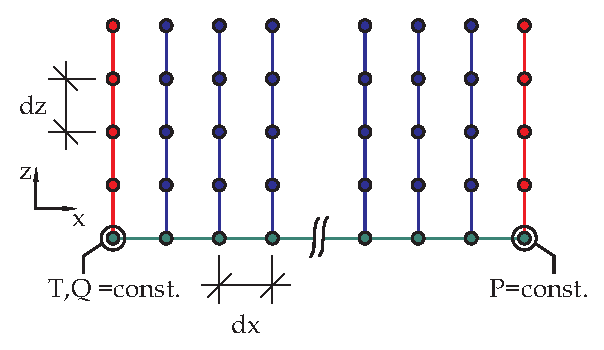
\includegraphics[width=0.65\textwidth]{T/figures/lauwerier-grid.eps}
\caption{\label{fig-lauwerier-grid}Alignment of the grid for the numerical model.}
\end{figure}
Fig.~\ref{fig-lauwerier-scheme} shows the positions of observation points which were chosen to evaluate the numerical model by the comparison with analytical solutions. 
\begin{figure}[h]
\centering
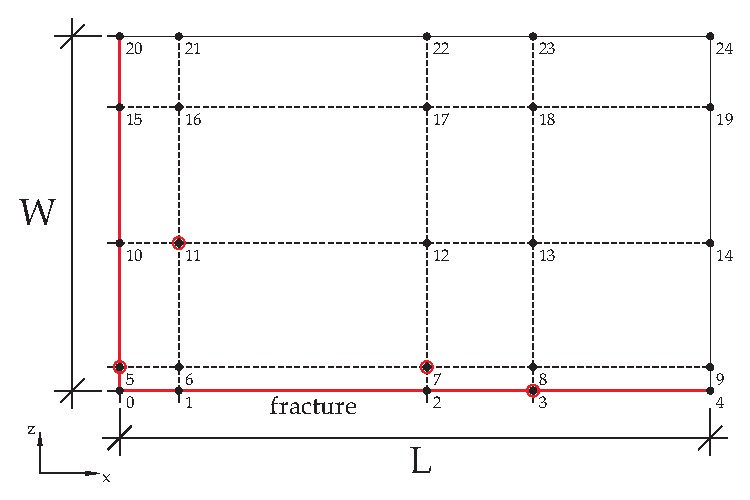
\includegraphics[width=0.65\textwidth]{T/figures/lauwerier-scheme.eps}
\caption{\label{fig-lauwerier-scheme}Positions of observation points for temperature breakthrough curves.}
\end{figure}

\subsection{Parameters}

The chosen parameters and material properties for this solution are shown in Tab.~\ref{tab-lauwerier-parameters}.
\begin{table}[ht]
\caption{\label{tab-lauwerier-parameters}Model parameters for the \textsc{Lauwerier}-problem.}
\begin{center}
\begin{tabular}{llll}
\toprule
parameter 						& value \\
\midrule
\multicolumn{2}{c}{\textit{spatial discretisation}} \\
fracture length $L$				& $\unit[50]{m}$  \\
matrix width $W$ 				& $\unit[63.25]{m}$  \\
step size X $\Delta x$ 			& $\unit[2]{m}$  \\
step size Z $\Delta z$ 			& $\unit[0.1265]{m}$  \\
half of fracture width $b/2$ 	& $\unit[1.0 \cdot 10^{-3}]{m}$  \\
groundwater velocity $v_x$ 		& $\unit[1.0 \cdot 10^{-4}]{m/s}$ \\
\cmidrule{1-4}
\multicolumn{2}{c}{\textit{temporal discretisation}}\\
timesteps $\Delta t$ 			& $\unit[2.0 \cdot 10^{5}]{s}$  \\ 
No. of timesteps 				& 2500 \\
total time 						& $\unit[5.0 \cdot 10^{8}]{s}$  \\
\cmidrule{1-4}
\multicolumn{2}{c}{\textit{material properties -- solid}}\\
thermal conductivity $\lambda$ 	& $\unit[1]{W \cdot m^{-1} \cdot K^{-1}}$  \\
heat capacity $c$ 				& $\unit[1000]{J \cdot kg^{-1} \cdot K^{-1}}$  \\
density $\rho$ 					& $\unit[2500]{kg \cdot m^{-3}}$  \\
\cmidrule{1-4}
\multicolumn{2}{c}{\textit{material properties -- fluid}}\\
heat capacity $c$ 				& $\unit[4000]{J \cdot kg^{-1} \cdot K^{-1}}$  \\
density $\rho$ 					& $\unit[1000]{kg \cdot m^{-3}}$  \\
\bottomrule
\end{tabular}
\end{center}
\end{table}

\subsection{Results}

The quality of the numerical results can be shown by temperature distribution curves for several times in the rock matrix. Fig.~\ref{fig-lauwerier-rock} shows the temperature profiles for $x=\unit[0]{m}$ at three moments $t'$. The numerical solution has a very good agreement to the analytical results. Temperature profiles along the fracture at $z=\unit[0]{m}$ are plotted in Fig.~\ref{fig-lauwerier-fracture}. For long simulation times ( $t'=1000; t'=600$) both solutions fits very well together. For short simulation times, the numerical solution differ slightly from the analytical results. This discrapancy for short simulation times can be examined in Fig.~\ref{fig-lauwerier-points}, where temperature breakthrough cures for certain points (see Fig.~\ref{fig-lauwerier-scheme}) is plotted.
\begin{table}[h]
\caption{Benchmark deposit.}
\begin{center}
\begin{tabular}{lll}
\toprule
Deposit & Version & Date \\
\midrule
T$\backslash$Lauwerier$\backslash$Lauwerier & 4.7.03 & Jul.~2008 \\
\bottomrule
\end{tabular}
\end{center}
\end{table}
\begin{figure}[H]
\centering
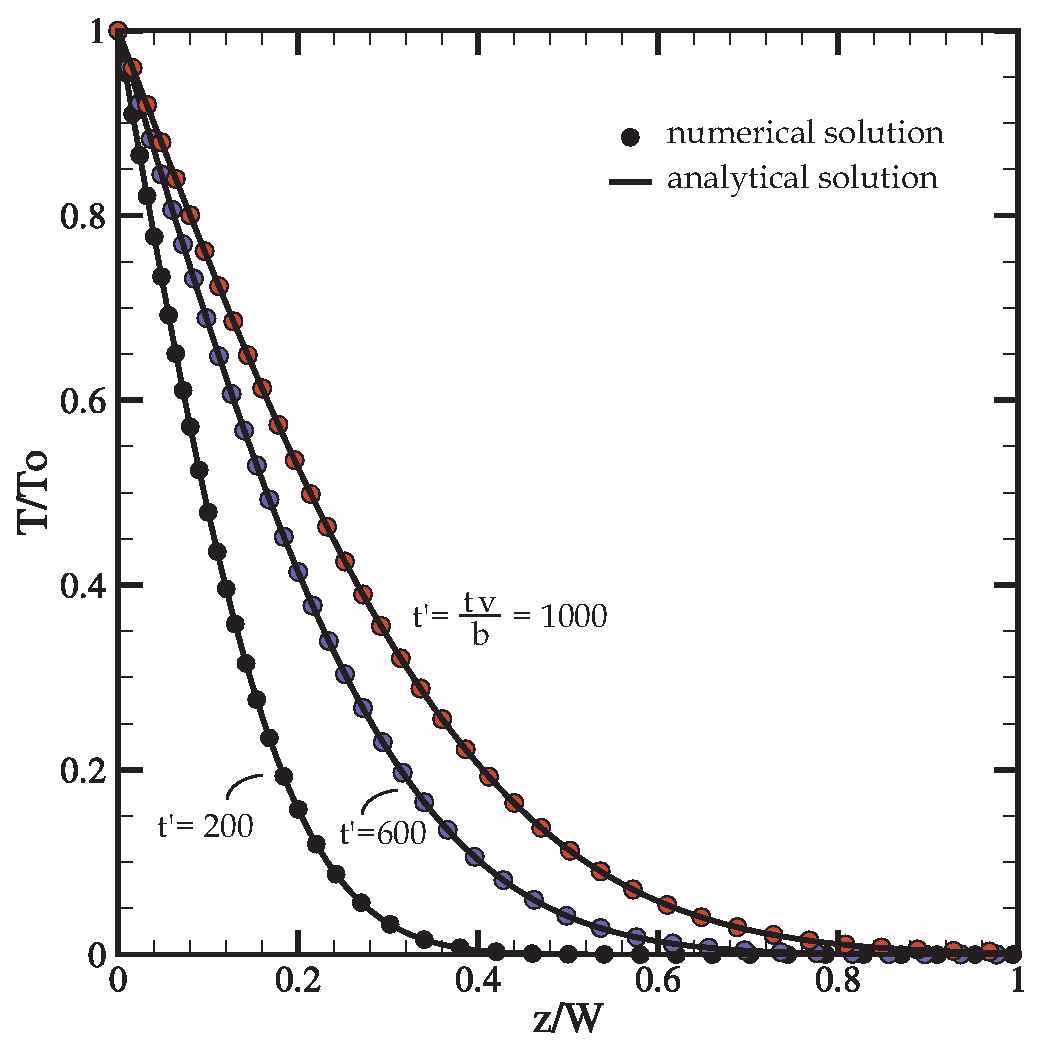
\includegraphics[width=0.6\textwidth]{T/figures/lauwerier-rock.eps}
\caption{Temperature distribution orthogonal to the fracture at $x=0$ at three different times.}
\label{fig-lauwerier-rock}
\end{figure}
\begin{figure}[H]
\centering
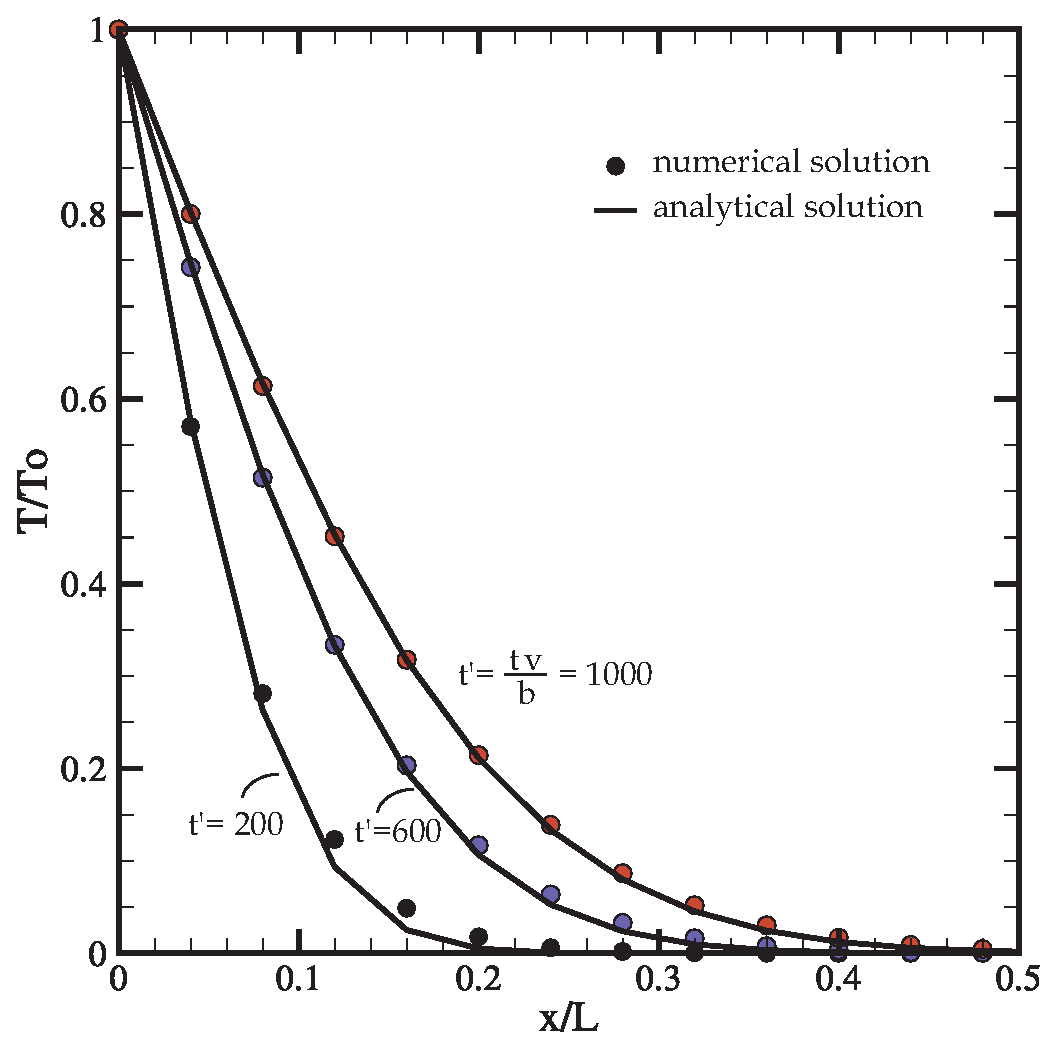
\includegraphics[width=0.6\textwidth]{T/figures/lauwerier-fracture.eps}
\caption{Temperature distribution along the fracture at three different times.}
\label{fig-lauwerier-fracture}
\end{figure}
\begin{figure}[H]
\centering
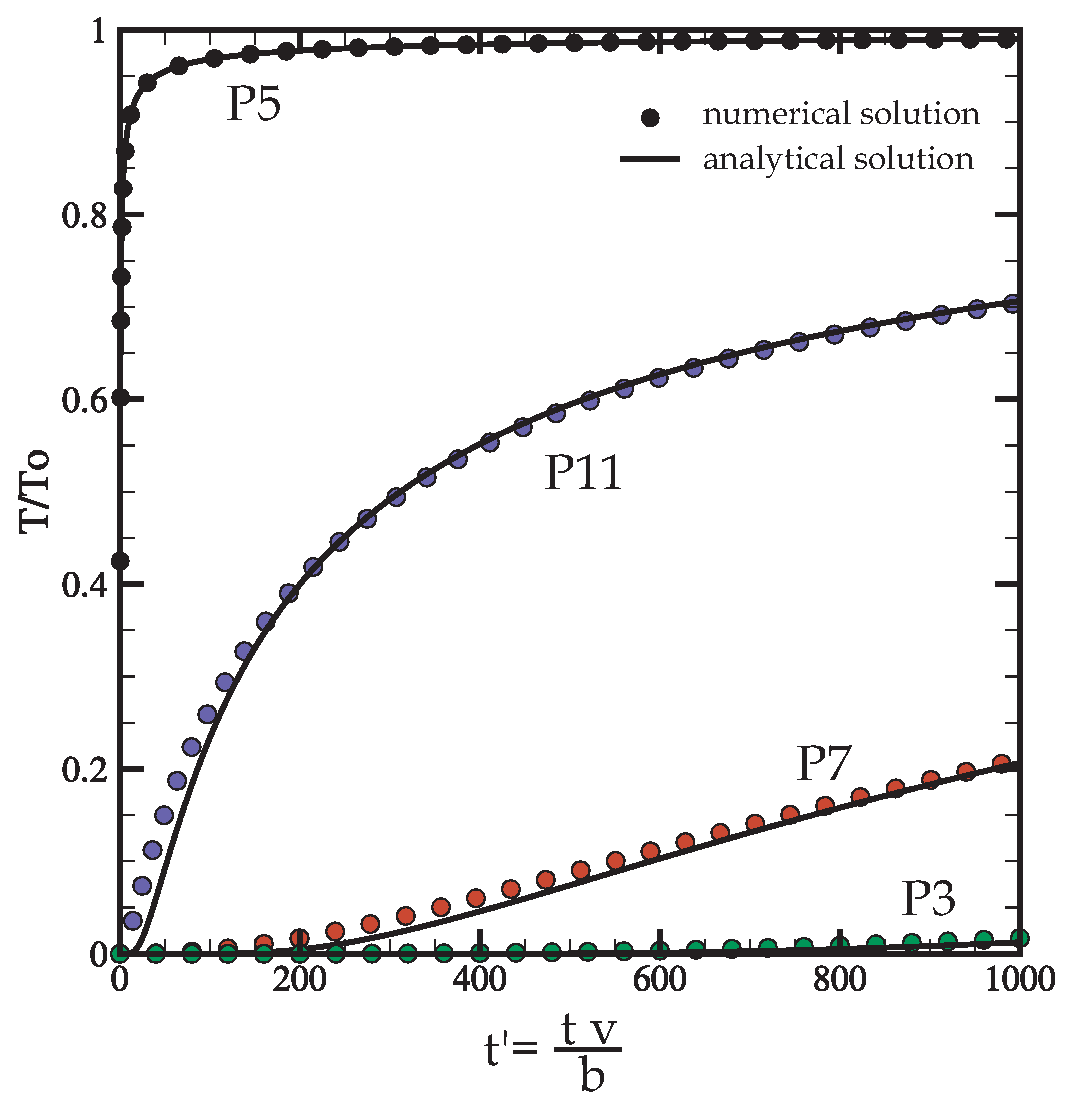
\includegraphics[width=0.6\textwidth]{T/figures/lauwerier-points.eps}
\caption{Temperature breakthrough curves at certain points in the rock matrix.}
\label{fig-lauwerier-points}
\end{figure}
%\clearpage